\documentclass{article}
\usepackage[T1]{fontenc}
\usepackage{lmodern}
\usepackage{graphicx}
\usepackage{amsmath,amssymb}
\usepackage[a4paper,margin=2cm]{geometry}
\usepackage[absolute,overlay]{textpos}
\setlength{\TPHorizModule}{1mm}
\setlength{\TPVertModule}{1mm}
\usepackage[indonesian]{babel}
\usepackage{hyperref}
\setlength{\emergencystretch}{2em}
% unit: Halaman 36

\begin{document}

% === Halaman 36 (llm) ===

\textbf{5. Enkripsi (\textit{encryption}) dan dekripsi (\textit{decryption})}

\begin{itemize}
    \item Enkripsi: proses menyandikan plainteks menjadi cipherteks. \\ Nama lain: \textit{enciphering}
    \item Dekripsi: proses mengembalikan cipherteks menjadi plainteks semula. \\ Nama lain: \textit{deciphering}
\end{itemize}

\vspace{10mm}

% deskripsi: Diagram alur proses enkripsi dan dekripsi yang menunjukkan perubahan plainteks menjadi cipherteks melalui proses Enkripsi, kemudian kembali menjadi plainteks melalui proses Dekripsi.
% bbox normalisasi: [0.1540, 0.5560, 0.8080, 0.7140]
\begin{textblock*}{137.34mm}(32.34mm,165.13mm)
\noindent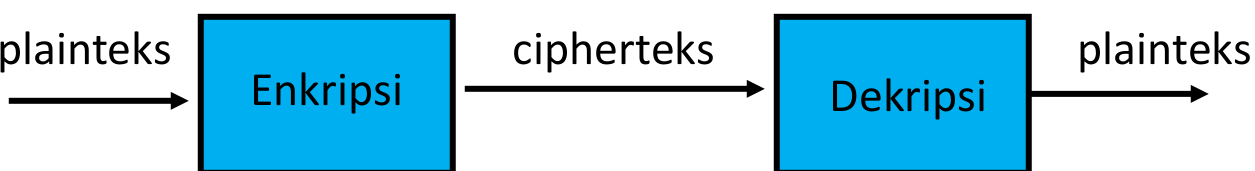
\includegraphics[width=137.34mm,height=46.93mm]{../../images/llm/page_036_img_01.png}%
\end{textblock*}

\end{document}
